
% 原文 p.359
\hypertarget{srcpage:359}{}\label{srcpage:359}
\sectionlink{観測、量子的な脳、デコヒーレンス}
\setcounter{footnote}{0}

生物系が量子力学的な言葉で分析されることは、めったにない。そのような系の途方もない複雑さのため、量子力学的に扱うことは本質的に不可能である。さらに、生物系の構造は通常、室温の水性環境に埋め込まれている。したがって、そのような系には非常に強いデコヒーレンスが働き、量子コヒーレントな振る舞いを実効的に抑制すると予想するのが合理的である。同時に、量子力学があらゆる尺度で妥当だと考えるなら、生物構造の振る舞いは量子力学の法則に従う。

この文脈で、脳は特に興味深い生物系である。それは私たちの知覚を処理する中枢の器官をなす。物理理論の経験的に意味のあるあらゆる言明は、まさにこれらの知覚に関係づけられなければならないことは明らかである。したがって、理論の予測に基づいて私たちの観測を説明しようとするとき、これらの知覚を私たちへもたらす系、すなわち脳の役割を説明する必要があるかもしれない。さらに、以下で概説するように、歴史的には、量子論における「意識」の役割という関連する問題も生じており、意識が波動関数の収縮を誘起するかもしれないという提案もなされてきた。

本章では、量子力学における観測の一般的問題について、いくつかの導入的考察を行った後（9.1節）、9.2節で、von Neumannの測定図式（2.5.1節参照）に観測者を明示的に含め、その帰結を論じる。続いて、量子力学的な脳に焦点を当てる（9.3節）。脳内のニューロンや、ほかの構造の重ね合わせ状態のデコヒーレンス特性を模型化した研究をいくつか述べる。それらからは、関係するデコヒーレンス時間尺度の具体的な数値評価が得られている。9.4節では、これらの結果が、測定問題の「主観的」解決に対して持つ含意も、簡単に論じる。

\subsectionlink{量子力学における観測者の役割}
量子力学における観測者の役割は、理論の初期にまでさかのぼる、多くの基礎論争の核心にあった。古典物理学とは対照的に、状態が本質的に壊れやすいという事実が、量子力学の特異な特徴であることを思い出そう（2.1節参照）。
% 原文 p.360
\hypertarget{srcpage:360}{}\label{srcpage:360}
ある特定の物理量の測定は一般に、系の量子状態を乱し、それゆえ非可換な観測量で表される、別の物理量の後続の測定結果を乱す。

したがって、系の物理状態は、観測者が測ることを選ぶもの、そのもので「ある」ように見える。この特徴は、古典理論ではほとんど知られていない「主観性」の色合いを、自然の記述へ持ち込む。ゆえに、観測、したがって観測者は、古典物理学におけるよりも、量子力学でははるかに根本的な役割を果たすように見える。「粒子の軌道は、私たちがそれを観測する行為によって作られる」\cite[185頁]{ref042}というHeisenbergの急進的な言明を、すでに引用した（原著19頁参照）。Bohrの著作に最も明瞭な、この実証主義的な見方では、量子力学の形式全体は本質的に、測定が行われた場合に、観測者が何を見いだすかを予測する処方箋をなす。しかし、「外部に実際には何があるか」について、存在論的主張は何も行わない。実際、Copenhagen解釈では、測定前の系の物理状態についての言明は、すべて無意味とされる。

実験物理学の実用的な問題を扱う際には、Copenhagen解釈の何らかの変種を採用する多くの人々でさえ、量子力学が指示すべき、観測者に依存しない物理的実在の存在を信じ続けている。そこで中心となる問いは、物理系には一般に、測定前の物理量の値の完全な組を割り当てられない、という量子力学から学んだ教訓を、理論が何らかの仕方で関係してほしいと願う、私たちを取り巻く「客観的に存在する」世界への、直観的に感じられる必要性と、どう両立させるかである。

同時に、私たちは、単に主観的知覚の産物かもしれないにもかかわらず、客観的であり、したがって物理理論に必須の一部だとみなすようになった概念も、注意深く吟味することを迫られる。von Neumann\cite[第VI章]{ref060}は、次のことを思い起こさせた。
\begin{quote}
経験が述べるのは、「ある観測者が特定の主観的観測を行った」という種類の言明だけであり、「ある物理量が特定の値を持つ」という種類の言明では決してない\footnote{ドイツ語原文は次のとおりである。``Denn die Erfahrung macht nur Aussagen von diesem Typus: ein Beobachter hat eine bestimmte (subjektive) Wahrnehmung gemacht, und nie eine solche: eine physikalische Größe hat einen bestimmten Wert.''}。
\end{quote}
同様に、d'Espagnat\cite[134--135頁]{ref496}は、次のように注意を促す。
\begin{quote}
私たちが、別々の場所にある巨視的物体というような「もの」を知覚するという事実は、少なくとも部分的には、私たちの感覚と知性の装置の構造による。したがって、それを、量子状態を定義するために考慮しなければならない、確かな知識の総体の一部とみなすべきではない。（中略）実際、科学の目的は、人間の経験を記述することであって、「実際にあるもの」を記述することではない、と科学者が主張するのは、まったく正しい。そして、人間の経験を記述したいだけである限り、すなわち、すべての可能な状況で何が観測されるかを予測できることで満足する限り、（中略）通常の三次元空間の確定した場所に、観測されていない、すなわちまだ観測されていない物体が、何らかの絶対的意味で存在すると仮定する必要はない。
\end{quote}

% 原文 p.361
\hypertarget{srcpage:361}{}\label{srcpage:361}
したがってvon Neumannとd'Espagnatは、一般的で客観的な「確定性」に対する、しばしば深く感じられるこだわりが、巨視的な系についての日常経験だけに基づいていることを認識するよう促している。もし経験とは独立に、確定性が自然界に実際に存在することを知ることができるなら、「外部」の物理現象を「内部」の知覚・認知装置へ結びつける単純な模型を作りさえすれば、主観的確定性は、おそらく客観的確定性の帰結になるだろう。その模型が単純であると予想する根拠としては、外部過程と内部過程を支配する物理法則が同一だという想定を挙げられる。von Neumannは、この仮定を「心身並行論」\cite{ref060}と呼んだ。しかし、どの知識も直接または間接に観測に基づくので、確定性の客観的存在についての知識を、私たちの主観的な確定性の観測に根ざさせずに得る方法はない。同時に、巨視的な干渉・コヒーレンス現象は、量子世界と、直接経験の水準で観測される確定性との境界が、曖昧であることを明瞭に示している（第6章参照）。

したがって、満足のいく物理理論には、客観的確定性が先験的な一部として含まれるべきだという要求を捨てることも、実際には合理的かもしれない。もちろん、その理論が、私たちが主観的に観測するすべての確定性を、経験と一致するように説明できることが条件である。それに対応する測定問題の「主観的」解決は、デコヒーレンス理論から大きな後押しを受けてきた。実際、デコヒーレンスは、この種の主観的方法の多くを、そもそも経験的に成立可能にする。全体の水準で確定性を強制しなくても、局所観測者の視点から確定性を導けるかもしれないからである。後の9.4節で、このような方法をより詳しく論じる。

\subsectionlink{量子的観測者とvon Neumann連鎖}
Copenhagen解釈（8.1節）や、ほかの量子力学の解釈のように、測定と観測者へ特定の先験的役割を与える代わりに、ここでは異なる視点を取ろう。観測者を単に、観測対象の系と相互作用する量子系として扱う。この状況は、2.5.1節で論じたvon Neumannの測定図式を用い、観測者を、測定相互作用のvon Neumann連鎖における最後の環として含めて模型化できる（図9.1）。


% 原文 p.362
\hypertarget{srcpage:362}{}\label{srcpage:362}
\begin{figure}[htbp]
\centering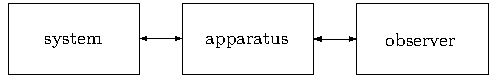
\includegraphics[width=.88\linewidth]{figures/ch09_fig01.pdf}
\caption{最後の環として観測者を含めたvon Neumann連鎖。}
\end{figure}

このとき、測定の異なる可能な結果を観測することに対応する、観測者の量子状態は、測定装置の対応する相対状態と量子的に相関する。さらに装置は、対象の系を記述する重ね合わせ状態の異なる成分と量子的に相関する。この測定相互作用を、通常のvon Neumannの形で模式的に表すと、次のようになる［(2.54)参照］。
\begin{equation}
\begin{aligned}
&\Bigl(\sum_n c_n|n\rangle\Bigr)|\text{装置準備完了}\rangle|\text{観測者準備完了}\rangle\\
&\quad\longrightarrow\sum_n c_n|n\rangle|\text{指針は }n\rangle|\text{観測者が結果 }n\text{ を知覚}\rangle .
\end{aligned}\tag{9.1}
\end{equation}
ここで$\sum_n c_n|n\rangle$は、観測、すなわち測定される系の状態である。したがって、この形式で測定を記述する最終量子状態は、系・装置・観測者がもつれた重ね合わせ状態であり、その各成分は、測定の異なる「結果」に対応する。

しかし、(9.1)のように観測者を含めても、相互作用する系のvon Neumann連鎖は終わらない。この連鎖に、環境、二次的装置や観測者など、さらに環を付け加えると、(9.1)と同様に、可能なすべての結果に対応する状態を含む、もつれた最終状態へ再び至る。これらの環をすべて含む複合系の時間発展が厳密にユニタリーである限り、この状態に含まれる情報量、たとえば純粋度やvon Neumannエントロピー（2.4.3節参照）で測られる情報量は変化できず、連鎖は終わらない。ゆえに、私たちは無限後退の問題に直面する。

ここから、これらの異なる相関した成分状態が、観測者が実際に経験する単一の測定結果へ、どのように、いつ縮約し得るのかという、根本的な問いが生じる。von Neumann連鎖が終わるのか、どのように、どこで終わるのかという問題は、もちろん本質的には結果の問題であり、本書のいくつかの箇所ですでに論じてきた（たとえば2.5.4節と8.1節参照）。von Neumann自身も、この問題を明確に認識していた。彼にとって唯一確かな事実は、観測者である私たちが、測定の終了時には常に確定した結果を知覚することだった。したがって理論は、少なくとも観測者の経験の水準で、そのような確定した知覚を説明しなければならない。量子力学の統計的予測は、観測連鎖のどこにHeisenberg切断を置くかに依存しない。
% 原文 p.363
\hypertarget{srcpage:363}{}\label{srcpage:363}
したがって、何らかの形の波動関数の収縮を、装置と観測者の間の、どの段階にも導入できる。しかし、明白な経験的制約によって、明らかに確定した結果を知覚することの説明が、実際に不可避となるのは、観測者の水準においてだけである。

この精神に沿って、von Neumannは観測者の内部での波動関数の収縮を仮定し、それを「第一の介入」（ドイツ語で``erster Eingriff''）と呼んだ\footnote{興味深いことに、系・装置・観測者の相互作用を支配するユニタリーなSchrödinger発展は、「第二の介入」と呼ばれた。}。この方法は、Copenhagen解釈（8.1節参照）と著しく対照的だった。後者では、量子力学的にそれ以上分析すべきではない、本質的に古典的な測定装置の存在という仮定の中に、波動関数の収縮が暗黙に含まれていたのに対して、von Neumannは、測定装置自体に特別な役割を与えなかった。しかし、相互作用する量子系という純粋に量子力学的な形式から、確定した結果の知覚をどう説明するかという問題を解決できず、彼は、基本的な量子・古典境界を維持せざるを得ないと感じた。ただし、その境界を今や観測者にまで押し進めたのである。したがって、測定過程を純粋に量子力学的に記述しようというvon Neumannの野心的目標は、観測者の水準での収縮を恣意的に導入したことで、途上で打ち切られたといえる。

von Neumann自身は、観測者における収縮の本性や、測定装置のような無生物と観測者とを何が区別するのかについて、詳しく述べなかった。しかし、Heisenberg切断を観測者の中に置くことによって、新たな扉が開かれた。すなわち、量子測定過程と、実際の、あるいは単に知覚されるだけの波動関数の収縮における、「意識」の役割という問いである。

物理理論の基本的水準に「心」や「意識」といった、かなり曖昧な言葉を含める方法は、確かに自然科学一般、特に物理学の伝統的方法に反する。同時に、量子論における観測者の特異な重要性、すなわち、私たちが直接観測する世界と同様の構造を持つ、観測者に依存しない実在という、それまで疑われなかった仮定から離れなければならないように見えることは、観測者の心に特別な物理的役割を与える考えを、再導入したように見える。

Copenhagen解釈自体と、そこに体現された実証主義的態度さえも、量子力学を本質的に、観測者による検証、すなわち測定の文脈で初めて物理的意味を得る言明の組とみなすことによって、「心」という概念に暗黙に重要性を与えている。d'Espagnat\cite{ref497}が論じたように、「ある」ものではなく、観測者が「見いだせる」ものだけに言及することによって、検証し、見いだす観測者の心が、科学的実在に先立つ原始的な概念をなす。
% 原文 p.364
\hypertarget{srcpage:364}{}\label{srcpage:364}
しかし、「心」や「意識」のような言葉は、Copenhagen解釈の明示的な一部ではなかった。また、観測者が得る知識は、それでも何らかの基礎的な物理的実在に関係しなければならない、という基本的直観を、この解釈の支持者は本当に捨てたわけではなかった。

意識が量子測定過程で基本的役割を果たすという考えの、有名な、ただし一時的な支持者にEugene Wignerがいた。彼の動機は、1960年代初頭に考案し、その後「Wignerの友人」の問題として知られるようになった思考実験\cite{ref498}に基づいていた。この思考実験は、Schrödingerの猫の設定を変えたものである。毒を、不安定な原子が崩壊すると閃光を発する測定装置に置き換え、決定的なこととして、猫を「Wignerの友人」と呼ばれる人間の観測者で置き換える。友人と区別するため、元のSchrödingerの猫の設定における外部観測者を、「Wigner」と呼ぼう。

したがって、この設定には二人の人間の観測者が含まれる。一人は、原子と装置の系との測定型相互作用が、von Neumann図式で量子力学的に記述される「内部」の観測者、すなわちWignerの友人である。もう一人は、後になってこの相互作用の結果を尋ねる「外部」の観測者、すなわちWigner自身である。猫、不安定な原子、毒を入れた元の猫の設定の箱は、ここでは原子、測定装置、Wignerの友人を含む実験室に対応する。Wignerは、しばらく実験室の外で待つ。その間に、原子・装置・Wignerの友人の結合状態は、通常の猫型の重ね合わせへ発展する。この発展を、模式的に次の形で表せる。
\begin{equation}
\begin{aligned}
&(\alpha|\text{原子未崩壊}\rangle+\beta|\text{原子崩壊}\rangle)
\otimes|\text{装置準備完了}\rangle|\text{観測者準備完了}\rangle\\
&\quad\longrightarrow\alpha|\text{原子未崩壊}\rangle|\text{閃光なし}\rangle|\text{閃光を観測せず}\rangle\\
&\qquad\quad+\beta|\text{原子崩壊}\rangle|\text{閃光あり}\rangle|\text{閃光を観測}\rangle .
\end{aligned}\tag{9.2}
\end{equation}
その後Wignerは、実験の結果を尋ねるために部屋へ入る。彼は友人に、閃光を見たかどうか尋ねる。友人は明らかに、閃光を観測したか、観測しなかったかの、どちらかを答える。その答えに応じてWignerは、自分の視点からは、原子・装置・友人の結合系を記述する猫状態が、(9.2)の右辺の二成分の一方へ収縮したと結論するだろう。しかし、彼が実験室へ入って最初の問いを発する前の、閃光に関する経験を尋ねたら、Wignerの友人は何と答えるだろうか。

本質的には、Schrödingerの猫の設定の場合と同様、Wignerの友人の例が浮き彫りにする中心的問題は、収縮を誘起する測定が、いつどこで行われるかという問いである。
% 原文 p.365
\hypertarget{srcpage:365}{}\label{srcpage:365}
ただし、Wignerの友人の場合には、Schrödingerの猫の逆説との違い、そしてWignerの考えでは決定的な違いは、重ね合わせが意識ある観測者を含むことである。この観測者は、Wignerが実験室へ入って閃光を見たかどうかを尋ねる前の経験について、彼が部屋に入った後、言葉による報告を与えられるはずである。

Wigner自身は、(9.2)の二つの異なる「意識状態」、すなわち閃光の観測に対応する状態と、閃光を観測しない状態の重ね合わせは、不合理だとみなさなければならないと考えた。彼の意見では、意識ある観測者は、常にこれらの状態の一つだけにいなければならなかった\cite{ref498}。この信念から彼は、意識的観測は(9.2)のような標準的な線形量子形式では記述できないと結論した。すなわち、意識は、ユニタリー発展を破り、意識ある観測者の確定した状態への波動関数の収縮を誘起するという意味で、物質的対象と根本的に異ならなければならないとした。

純粋に経験的な観点からは、Wignerの推論の決定性に対する強い反論がある。異なる意識状態の重ね合わせは、これらの状態がいかなる仕方でも干渉しない限り、すなわち意識ある観測者の異なる「量子的版」が互いを「意識」しない限り、必ずしも不合理とみなして排除する必要はない、ということである。デコヒーレンスは、意識ある観測者にも避けがたく影響する。したがって、観測者の「内側からの見方」では、(9.2)の異なる「意識の分枝」の存在を、経験的に確認することはできないだろうと推測できる。この点は、9.4節でより詳しく論じる。実際Wignerは、デコヒーレンス研究の基礎となる考えのいくつかを導入した、Zehの1970年の論文\cite{ref004}を知ると、後に、量子測定における意識の特別な役割という見解を捨てた\cite{ref499}。

\subsectionlink{脳におけるデコヒーレンス：脳は量子コンピューターか}
脳は、$O(10^{11})$個のニューロンが$O(10^{14})$個のシナプスで相互接続された、驚くほど複雑なネットワークからなる。この神経回路網の記憶能力と動的相互作用が、感覚入力の保存と処理の生理学的核心であることを示す、説得力ある議論がある。「意識」の知覚を含む、すべての認知過程が、最終的にはニューロン活動へ還元できると推測することは、不合理ではない。神経生物学や生物物理学の研究者は、脳を通常、オン・オフの「スイッチ」（節点）が大規模に並列接続された網として、完全に古典的な言葉で模型化する\cite{ref500,ref501,ref502}。各節点は単一のニューロンを表し、特定の、しばしば非線形な活性化関数に応じてオンまたはオフとなり、それぞれニューロンの発火状態と静止状態に対応する。明白な理由から、このような模型は通常、人工神経回路網と呼ばれる。


% 原文 p.366
\hypertarget{srcpage:366}{}\label{srcpage:366}
大まかにいえば、このように脳は古典コンピューターとして模型化される。そのような模型研究から得られた意外な知見の一つは、比較的少数の節点と、各節点の活性化に関するごく少数の規則だけに基づく、比較的単純なネットワークでさえ、単純な認知過程で観測されるものに似た、驚くほど複雑な振る舞いを生み出せることである。しかし、このような古典模型の成功にもかかわらず、量子効果が私たちの認知装置で重要な役割を果たすかどうかは、少なくとも二つの観点から論じられてきた。

第一に、量子的な「不確定性」と、量子力学の見かけ上の非決定性を持ち出して、古典物理学が要請する厳密な決定論を回避し、「自由意志」という概念を回復しようとすることがある。しかし、この方法には根本的な誤りがある。どのような量子的「不確定性」も、まったく制御不可能な効果を表すはずであり、自分の行動を能動的に制御し決定できるという感覚に基づく、「自由意志」の理解とは完全に異なる。同じ理由で、量子力学が測定結果の確率だけを予測し、それゆえ物理世界の記述に非決定性を再導入するように見えるという事実から、自由意志の存在を推論することはできない。繰り返せば、そのような「量子的ランダムさ」が引き起こす行動は、自由意志を持つとされる個人には制御できない。したがって、このように量子論を持ち出すことは、何かをもたらすとしても、古くからの「自由意志の問題」を、もしそれがそもそも問題であるなら、いっそう深刻にするだけである\footnote{自由意志について、Einsteinは1932年の思索的な『Credo』\cite{ref503}で、かつて次のように述べた。「私は自由意志を信じない。Schopenhauerの『人は自分の欲することを行うことはできるが、自分の欲することを欲することはできない』という言葉は、生涯のあらゆる状況で私に付き添い、他人の行いが私にとってかなり苦痛であるときでも、それを受け入れさせてくれる。自由意志がないと知ることは、行動し判断する個人としての自分自身や同胞を、あまり深刻に受け取りすぎたり、平静を失ったりすることから、私を守ってくれる。」原文は次のとおりである。``Ich glaube nicht an die Freiheit des Willens. Schopenhauers Wort: `Der Mensch kann wohl tun, was er will, aber er kann nicht wollen, was er will', begleitet mich in allen Lebenslagen und versöhnt mich mit den Handlungen der Menschen, auch wenn sie mir recht schmerzlich sind. Diese Erkenntnis von der Unfreiheit des Willens schützt mich davor, mich selbst und die Mitmenschen als handelnde und urteilende Individuen allzu ernst zu nehmen und den guten Humor zu verlieren.''}。最後に、脳内のシナプス伝達には、その基礎にある生物過程の複雑さのために、かなり高い失敗率があることにも注意すべきである\cite{ref504}。これによって、「日常の水準」で、かなり高い予測不可能性が必然的に生じる。このような純粋に機能的な予測不可能性は、どのような量子的不確定性の効果よりも、おそらくはるかに重要である。したがって、予測可能な入出力パターンを持つ、決定論的な古典コンピューターとして脳を見ることは、実際にはあまり文字どおりに受け取るべきではない。


% 原文 p.367
\hypertarget{srcpage:367}{}\label{srcpage:367}
量子論を脳へ適用するこの「素朴な」考えを超えたところには、脳が生み出す人間の認知過程の複雑さは、脳が量子コンピューターとして働くことができる場合にだけ説明できるかもしれない、という提案の領域がある。言い換えれば、こうした提案は、脳の能力の少なくとも一部が、脳内の通常の古典状態、たとえばニューロンの静止状態と発火状態の、量子コヒーレントな重ね合わせの存在と操作によるかもしれない、という考えに基づく。もしこれが正しければ、古典的な人工神経回路網では、脳を完全にシミュレートするには本質的に不十分だということになる。

特に、人間の意識が量子コヒーレントな過程に結びついているかどうかは、しばしば論じられてきた。前の9.2節では、関連しているが向きの逆の概念、すなわち意識の作用が波動関数の収縮を引き起こすかもしれないという、Wignerの初期の推測\cite{ref498}に、すでに触れた。そこでは、測定型相互作用のvon Neumann連鎖によって作られた、全体のもつれた状態(9.1)に含まれる量子コヒーレンスを、実効的に破壊するために意識が持ち出された。今や問題の向きは逆である。量子コヒーレンスは、意識の出現に結びついているのだろうか。この文脈では、さまざまな巨視的量子コヒーレント過程が、意識の起源として提案されてきた（たとえば\cite{ref505,ref506,ref507,ref508,ref509,ref510,ref511}参照）。特に著名なのは、Penrose\cite{ref473}たち\cite{ref512,ref513,ref514}による提案である。彼らは、細胞骨格、すなわち細胞内部の足場の主要部分をなす、動的に活動する構造である、脳内のいわゆる微小管が、量子計算を可能にするほど長いデコヒーレンス時間を持つかもしれず、さらに、その計算が意識の出現と結びつくかもしれないと提案した（後の9.3.2節参照）。

意識というかなり曖昧な概念や、基礎物理理論におけるその役割の可能性に関する問題とは、まったく独立に、ここで論じるべき明白な中心的問いは、次のものである。脳内の関係する構造、特にニューロンと微小管は、脳内で量子計算を実行できるほど長く、量子コヒーレンスを維持できるだろうか。本書の前の章でのデコヒーレンスの議論に基づけば、そのようなデコヒーレンス時間は極めて短いと予想するだろう。結局、ニューロンと微小管は、生物学的尺度では小さくても、量子物理学で通常考える尺度では、依然として巨視的で非常に複雑な物体である。たとえばニューロンが発火と静止の重ね合わせにある状態は、巨視的に異なる状態の重ね合わせという分類へ、明らかに入る（以下参照）。さらに、これらの構造は、巨視的な「暖かく湿った」環境に埋め込まれ、その環境と強く相互作用している。

デコヒーレンス時間の短さについてのこの直観は、Tegmarkが2000年に報告した定量的結果\cite{ref515}によって支持された。Tegmarkは、ニューロンと微小管が脳内の自然な環境と相互作用する模型を考え、これらの構造における重ね合わせ状態のデコヒーレンス時間尺度について、桁の評価を示した。
% 原文 p.368
\hypertarget{srcpage:368}{}\label{srcpage:368}
以下の9.3.1節でニューロンのデコヒーレンスを、9.3.2節で微小管のデコヒーレンスを扱い、これらの結果を述べる。測定問題の「主観的」解決に対する含意は、9.4節で論じる。

\subsubsectionlink{ニューロンの重ね合わせ状態のデコヒーレンス時間尺度}
まずTegmark\cite{ref515}が考えた、ニューロンのデコヒーレンスを論じよう。ここで関心のあるニューロンの主要部分は、いわゆる軸索である。これは、直径約$d\approx10\,\mu\mathrm m$の、長い中空の管と考えられる（図9.2）。軸索壁の大部分は、絶縁体として働くミエリンで覆われている。しかし、軸索に沿って、この絶縁がない幅数nmの狭い帯があり、厚さ約$h\approx10\,\mathrm{nm}$の半透膜の領域を形成する。そこでは、軸索の内部と、それを取り囲む水性媒質との間で、イオンが交換される。ニューロンの発火は、膜内に位置する電位依存性Naチャネルを介して、周囲からこれらの膜領域を通り、軸索内部へNaイオンが非常に急速に流入することによって表される。この発火は、軸索に沿って最大$100\,\mathrm{m/s}$という高速で伝播し、各領域のNaチャネルを開く。イオンの流入は約1msしか続かず、その後Naチャネルは再び閉じ、ニューロンは静止状態へ戻る。中枢神経系に見られるニューロンの典型的パラメーターを使い、Tegmarkは、発火中に、個々の膜領域すべてからの寄与を合わせた軸索膜全体を、合計$O(10^6)$個のNaイオンが横切ると見積もった。

\begin{figure}[htbp]
\centering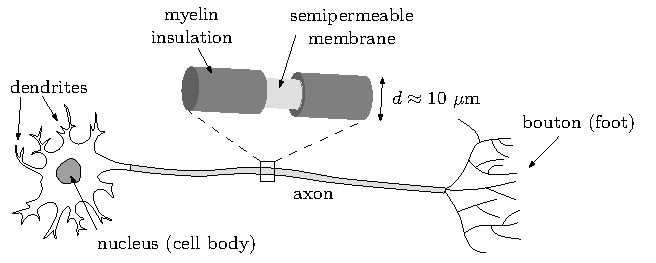
\includegraphics[width=.94\linewidth]{figures/ch09_fig02.pdf}
\caption{ニューロンの模式図。説明を明瞭にするため、軸索の一部分を拡大している。軸索壁の大部分はミエリンで覆われ、軸索内部を周囲の媒質から絶縁している。しかし、小さな帯状領域にはこの絶縁がなく、そこにある半透膜をイオンが通り抜けられる。}
\end{figure}

これは、発火中には静止中より、軸索内部に$N=10^6$個程度多くのNaイオンがあることを意味する（図9.3参照）。
% 原文 p.369
\hypertarget{srcpage:369}{}\label{srcpage:369}
したがって、発火状態と静止状態の重ね合わせは、$O(N)$個のNa原子の集まりが、それぞれ軸索の内部と外部に位置する二つの状態の重ね合わせに対応する。言い換えれば、$O(N)$個のNa原子からなる系を扱っており、それは$O(h)$の距離だけ離れた二つの重心位置の重ね合わせで記述される。

\begin{figure}[htbp]
\centering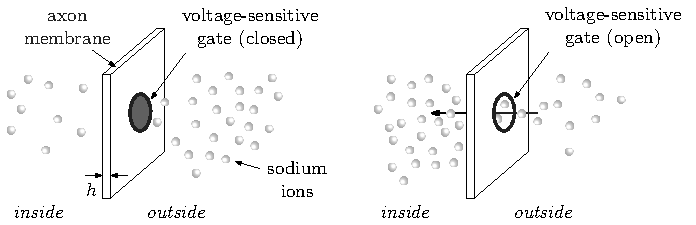
\includegraphics[width=.94\linewidth]{figures/ch09_fig03.pdf}
\caption{ニューロンの静止状態（左）と発火状態（右）。発火状態では、静止状態よりも$O(10^6)$個多くのNaイオンが軸索内部に存在する。}
\end{figure}

Tegmarkは次に、ニューロンの重ね合わせがコヒーレンスを失う、三種類の環境相互作用を調べた。すなわち、近くのNaイオンおよびKイオンとNa原子との衝突、周囲の水分子との衝突、離れたイオンとの静電的、すなわちCoulomb相互作用である。三つの場合はすべて、第3章で述べた散乱によるデコヒーレンスの理論を用いて扱える\footnote{第3章で作った模型は、散乱体、すなわち対象の系の運動量変化が、散乱される環境粒子の運動量変化に比べてはるかに小さく、物体の反跳を無視できるという仮定に基づいていることに注意しよう。厳密には、ここではこの近似は成り立たない。散乱体であるNaイオンの質量が、環境粒子であるNaイオン、Kイオン、水分子の質量と同程度だからである。したがって、以下の数値評価をあまり文字どおりに受け取るべきではない。他方、現在の目的には、いくつかの粗い評価で満足することにする。正しい値が、この評価から数桁ずれていても、ニューロンのこのような重ね合わせ状態のデコヒーレンス時間尺度が、生物学的・認知的過程に関係する時間尺度に比べて極めて短い、という一般的結論には影響しない。}。イオン同士の衝突と、イオンと水の衝突という、最初の二つの場合の考え方を、簡単に概説しよう。$T=310\,\mathrm K$、すなわち人間の体温における、NaイオンまたはKイオンと水分子の熱的de Broglie波長(2.114)は同程度で、$\lambda_{\mathrm{dB}}\approx0.03\,\mathrm{nm}$である。この値は、コヒーレントな空間的隔たり$h\approx10\,\mathrm{nm}$に比べてはるかに小さい。これは、散乱される環境粒子として働くイオンや水分子が、隔たり$h$を完全に分解できることを意味する。したがって、3.3.1節で論じた短波長極限に、完全に入っている。


% 原文 p.370
\hypertarget{srcpage:370}{}\label{srcpage:370}
デコヒーレンスが最大となるこの極限で、系の位置空間縮約密度行列の非対角要素の減衰率は、全散乱率$\Gamma_{\mathrm{tot}}$が定める値で飽和することを示した［(3.48)参照］。
\begin{equation}
\rho(x,x',t)=\rho(x,x',0)e^{-\Gamma_{\mathrm{tot}}t}.\tag{9.3}
\end{equation}
軸索の内側と外側にある重ね合わせ状態の、単一Naイオンについて、TegmarkはCoulomb散乱断面積を用い、NaイオンおよびKイオンとの衝突に対して$\Gamma_{\mathrm{tot}}\approx10^{14}\,\mathrm{s}^{-1}$、水分子の散乱に対してもほぼ同じ値と評価した。したがって、$N=10^6$個のイオンを含む空間的重ね合わせのデコヒーレンス時間尺度$\tau_{\mathrm d}$は、
\begin{equation}
\tau_{\mathrm d}=(N\Gamma_{\mathrm{tot}})^{-1}\approx10^{-20}\,\mathrm s\tag{9.4}
\end{equation}
程度と見積もられる。

より遠くのイオンとのCoulomb相互作用によるデコヒーレンスという第三の場合にも、Tegmarkは同様の散乱模型を使った。ここでは詳細に立ち入らないが、得られたニューロン重ね合わせの典型的なデコヒーレンス時間尺度の評価は、(9.4)と非常によく似ており、$\tau_{\mathrm d}\approx10^{-19}\,\mathrm s$である。すべての値を表9.1にまとめる。

\begin{table}[htbp]
\centering
\caption{Tegmark\cite{ref515}が報告した、ニューロンの発火・静止状態の重ね合わせと、微小管中のキンク状励起の重ね合わせについての、デコヒーレンス時間尺度の評価（秒）。}
\begin{tabular}{lll}\hline
対象&環境&デコヒーレンス時間尺度\\\hline
ニューロン&NaイオンとKイオン&$10^{-20}$\\
ニューロン&水分子&$10^{-20}$\\
ニューロン&離れたイオン&$10^{-19}$\\
微小管&離れたイオン&$10^{-13}$\\\hline
\end{tabular}
\end{table}

これらの値は、脳内の生物学的・認知的過程に関係する時間尺度と比べてどうだろうか。一回の発火の持続時間は$10^{-3}\,\mathrm s$程度であり、したがって$\tau_{\mathrm d}$より何桁も大きい。ゆえに、デコヒーレンスによって、発火の過程自体は実効的に古典的であると結論する。Tegmarkは、意図的行動、思考、発話、外部刺激への運動反応など、典型的な認知過程の時間尺度を、約$10^{-2}$から$10^0\,\mathrm s$と評価した。私たち自身の経験と、神経生理学の一般的な実験的証拠に照らして、これは確かに合理的に見える。そのような時間尺度が、ニューロンの重ね合わせについて評価された$10^{-19}$から$10^{-20}\,\mathrm s$というデコヒーレンス時間を、圧倒的に上回ることは明らかである。したがって、そのような重ね合わせは、上述の認知過程の例で重要な役割を果たせないと、かなり確実に結論できる。

さらに進んで、これらの結果から、何人かの著者が提案した、前述の「意識の量子的本性」についての知見を得ることもできる。すでに指摘したように、神経生物学の一般的証拠は、意識的知覚が、脳内の静止と発火の特定のニューロンパターンに結びついていることを示唆する。
% 原文 p.371
\hypertarget{srcpage:371}{}\label{srcpage:371}
Tegmark\cite{ref515}が論じたように、これは、次の理由により、意識が提案されているような量子的本性を持てないことを意味する。ある根本的な水準で、意識の源が実際に、十分長いデコヒーレンス時間を持つ脳の部分系に由来し、量子コヒーレントな過程が可能だと仮定できるとしよう。しかし、観測者の中に実際に意識的知覚を生じさせるには、この部分系は神経回路網と連続的に相互作用しなければならない。ニューロンは、その環境と強く結合しているから、部分系とニューロンの相互作用は、部分系内の量子コヒーレンスを急速に抑制し、したがって、提案された意識の量子的本性を実効的に破壊するだろう。この議論は、そのような量子的意識がどのような具体的形を取るかに、ほぼ依存しない。必要なのは、異なる意識的知覚は異なるニューロンの発火・静止パターンに対応する、という十分に動機づけられた仮定だけである。

最後に、ニューロンの関係する「計算」状態、すなわち静止状態と発火状態が、自然界で最も普遍的に見られる、環境によって超選択された状態、すなわち位置空間に局在した状態に対応するのは、もちろん偶然ではないことを指摘しよう。これらのニューロン状態は、環境相互作用にもかかわらず情報を頑健に符号化できる「記録状態」と同定できる\cite{ref067,ref104}（8.2.3節で概説したZurekの「実存的解釈」も参照）。もしニューロンの計算状態が、静止と発火の空間的重ね合わせに対応するなら、急速な散乱誘起デコヒーレンスを受けるため、脳内で情報を符号化するためには、ほとんど役に立たないだろう。

\subsubsectionlink{微小管の重ね合わせ状態のデコヒーレンス時間尺度}
Tegmarkは、微小管の重ね合わせ状態に対しても、典型的なデコヒーレンス時間尺度を評価した。原著367頁で述べたように、微小管は量子コヒーレントな動力学を可能にし、「人間の意識の起源」でさえあるかもしれないと提案されている\cite{ref473,ref512,ref513,ref514}。微小管は、脳のニューロンの主要成分であり、さまざまな細胞過程でも重要な役割を果たす。直径約24nm、長さが$\mu\mathrm m$からmm程度の、中空の円筒形をしている（図9.4）。各円筒は、いわゆるプロトフィラメント13本の束からなる。各プロトフィラメントは、$\alpha$チューブリンと$\beta$チューブリンという単量体から構成された、チューブリン二量体の線状配列である。$\beta$サブユニットは、余分な18個の$\mathrm{Ca}^{2+}$イオンを持ち、近傍の$\alpha$サブユニットには、同数の負電荷が位置する。これによって、二量体は強さ$36e$の電気双極子モーメントを持つ。各プロトフィラメントに沿って、ある二量体の$\alpha$サブユニットが、次の二量体の$\beta$サブユニットに接するように、チューブリン二量体が並ぶ。したがって、
% 原文 p.372
\hypertarget{srcpage:372}{}\label{srcpage:372}
物理学の観点では、プロトフィラメントは微小な電気双極子の鎖であり、平行に束ねられることによって、微小管全体としての正味の電気双極子モーメントを作り出す（図9.5）。

\begin{figure}[htbp]
\centering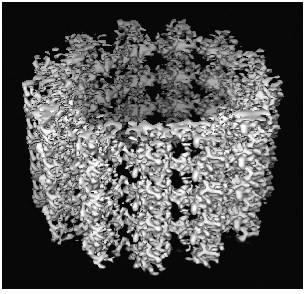
\includegraphics[width=.87\linewidth]{figures/ch09_fig04.pdf}
\caption{微小管の構造。約$8\,\text{\AA}$の分解能で得られた低温電子顕微鏡データに基づく、三次元再構成を示す。Lawrence Berkeley National LaboratoryのKen DowningのVisualization Groupが作成\cite{ref516,ref517}。}
\end{figure}
\begin{figure}[htbp]
\centering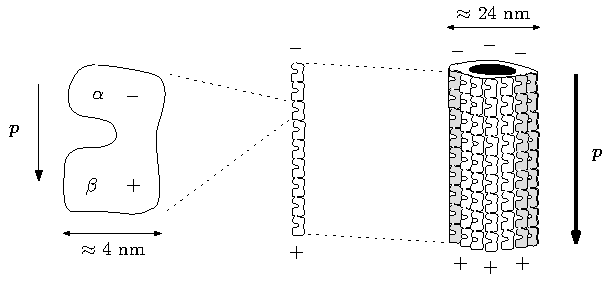
\includegraphics[width=.94\linewidth]{figures/ch09_fig05.pdf}
\caption{微小管の双極子モーメント。左：$\alpha$、$\beta$単量体からなる各チューブリン二量体は、小型の電気双極子として働く。中央：プロトフィラメントは、そのような電気双極子の鎖である。右：プロトフィラメントは、平行に束ねられて微小管を形成するため、微小管は個々のプロトフィラメントの双極子モーメントの和に等しい、双極子モーメントを持つ。}
\end{figure}

各二量体の内部には、非局在化した電子が一つ含まれ、それは、それぞれ$\alpha$サブユニット側と$\beta$サブユニット側にある、二つの疎水性ポケットのいずれかへ局在できる（図9.6）。
% 原文 p.373
\hypertarget{srcpage:373}{}\label{srcpage:373}
電子が$\beta$サブユニット側へ局在すると、二量体の$\beta$状態と呼ばれるが、二量体は、電子が$\alpha$サブユニット側に局在した立体配座、すなわち二量体の$\alpha$状態に対応する垂直軸から、約30度の立体配座変形を起こす。したがって、二量体は、立体配座状態$\alpha$と$\beta$に対応する基底状態を持つ、有効二状態系として記述できる。二量体が変形するため、電気双極子モーメントの向きは$\alpha$状態と$\beta$状態で異なり、これら二状態を、微小管軸方向の電気双極子モーメントの、二つの異なる値$p_\alpha$、$p_\beta$へ対応させられる。ゆえに、プロトフィラメントを、相互作用するIsingスピン$1/2$鎖の集合とみなせる。ここでは、スピンの「上」と「下」が、微小管軸方向の電気双極子モーメントの、二つの可能な状態$\alpha$と$\beta$に対応する。

\begin{figure}[htbp]
\centering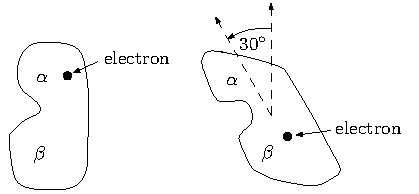
\includegraphics[width=.82\linewidth]{figures/ch09_fig06.pdf}
\caption{チューブリン二量体の二つの立体配座状態$\alpha$と$\beta$。}
\end{figure}

加水分解過程によるエネルギー供給のような、ある種の過程は、微小管の一端に位置するチューブリン二量体の、立体配座状態$\alpha$と$\beta$の間の変化を誘起できる\cite{ref518}。二量体間の双極子相互作用を介して、その二量体に付随する双極子モーメントの変化が、微小管軸に沿って高速に伝播する可能性が提案されている（図9.7参照）。Sataric、Tuszynski、Zakula\cite{ref519}は、微小管で損失なくエネルギーを輸送できる可能性を記述するため、そのような「キンク状」励起、すなわちソリトンの、詳しい理論模型を提案した。

\begin{figure}[htbp]
\centering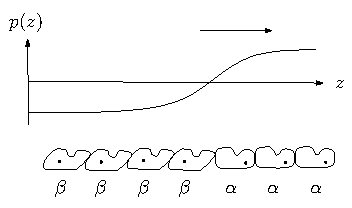
\includegraphics[width=.94\linewidth]{figures/ch09_fig07.pdf}
\caption{微小管中のキンク状励起の模型。微小管の一端で、チューブリン二量体の$\alpha$状態と$\beta$状態の間の立体配座転換に対応する、局所的双極子モーメントの変化が、二量体間の双極子相互作用を介して、微小管軸に沿って進む。これによって、微小管軸方向の双極子モーメント$p(z)$にキンク状励起が生じ、その励起が微小管軸に沿って高速で伝播する。簡単のため、ここでは$\alpha$状態と$\beta$状態を、微小管軸方向の電気双極子モーメントが、大きさは等しく向きが逆の値に対応させている。}
\end{figure}


% 原文 p.374
\hypertarget{srcpage:374}{}\label{srcpage:374}
Tegmark\cite{ref515}は、この特定の模型に焦点を当て、多数の二量体に相当する距離だけ離れた、二つのキンク状励起の重ね合わせについて、典型的なデコヒーレンス時間尺度を評価した。キンクの位置にある正味の電荷と、遠くの環境イオンとのCoulomb相互作用を考えた。その電荷は、微小管の断面をなす二量体の「輪」に含まれる、13個の$\beta$サブユニット中の、各18個の$\mathrm{Ca}^{2+}$イオンによる総電荷に等しいとした。十分離れた二つのキンクの重ね合わせのデコヒーレンス時間尺度$\tau_{\mathrm d}$は、遠くのイオンとの相互作用による、ニューロン重ね合わせのデコヒーレンスを模型化する際に使ったものと同様の、Coulomb散乱模型で評価された（9.3.1節参照）。Tegmarkは、$\tau_{\mathrm d}\approx10^{-13}\,\mathrm s$という値を得た（表9.1も参照）。微小管の量子コヒーレントな振る舞いの可能な本性を、この種の重ね合わせと同定するなら、Tegmarkの数値評価は、微小管が量子コンピューターのような量子コヒーレントな振る舞いを示す可能性を、かなり明瞭に排除する。

しかし、PenroseとHameroff\cite{ref473,ref512,ref513}が作った、かなり論争的な模型では、別の可能性が考えられている。ここでは、Tegmarkが調べた空間的に離れたキンク状励起の重ね合わせの代わりに、個々のチューブリン二量体の、二つの立体配座状態$\alpha$と$\beta$の重ね合わせを考える。微小管が量子コヒーレントな動力学を示すにはデコヒーレンスが強すぎる、というTegmarkの主張に異議を唱えるため、Hagan、Hameroff、Tuszynski\cite{ref514}は、個々の二量体を含むそのような配座の重ね合わせは、Tegmarkが評価したソリトンの重ね合わせのデコヒーレンス時間よりも、何桁も長いデコヒーレンス時間を可能にすると提案した。

$\alpha$状態と$\beta$状態の重ね合わせのデコヒーレンス時間を計算するため、Hagan、Hameroff、Tuszynski\cite{ref514}は、Tegmarkが使ったものと同様の模型を用いたが、それを単一二量体の双極子モーメントへ適用した。しかし、RosaとFaber\cite{ref520}が指摘したように、\cite{ref514}の計算における正当化できない近似を修正すると、得られるデコヒーレンス時間は、空間的に離れたキンク状励起の重ね合わせについて、Tegmarkがもともと与えた値と同程度になる。これらの評価は、Penrose--Hameroff型の模型を決定的に排除するものではないが、そのような理論に対する非常に重大な難題を提起する。

現在、大多数の研究者は、脳内の生物構造はおそらくデコヒーレンスを受けやす過ぎるため、認知過程や意識過程に関係する時間尺度にわたって、量子コヒーレンスを持続させることはできない、という見方を支持しているといってよい\cite{ref521}。したがって、脳の古典模型は、今日までほぼ揺るがされていない。Tegmarkの数値結果と、巨視的尺度でのデコヒーレンスについての一般的直観に基づけば、この状況が近い将来変わるとは考えにくい。


% 原文 p.375
\hypertarget{srcpage:375}{}\label{srcpage:375}
\subsectionlink{測定問題の「主観的」解決}
von Neumann連鎖の最終状態(9.1)は、観測者の異なる「心的状態」、すなわち$n$で区別される異なる結果の知覚に対応する状態が、装置、系などの相対状態と量子的に相関していることを記述する。そこで、測定問題の主観的解決を目指す方法は、全体の状態にコヒーレンスが存続しているにもかかわらず、可能な結果のうちただ一つだけを観測者が知覚することが、どのように生じ得るかを説明しようとする。この場合、「外部の物理的実在」が何であれ、それは全体の重ね合わせ状態(9.1)によって、完全に記述され続けてもよく、成分状態のどれか一つを選び出す経験的必要はない。9.1節で論じたように、理論が可能なすべての観測を正しく説明できるなら、このような測定問題の主観的解決を、満足のいく十分なものとみなすことを妨げる、根本的理由はない（\cite{ref001,ref322,ref496}も参照）。

上で述べたように、現在の科学的証拠は、すべてとはいわなくても大部分の認知活動、したがっておそらく観測者の「心の状態」ないし「心的状態」\footnote{以下の段落で引用符を頻繁に使うのは、「心」「意識」「心的状態」のような概念の、かなり曖昧な性格を、必然的に反映している。}が、脳内の神経回路網の特定の静止・発火パターンに結びつけられることを示唆する（知覚とニューロンパターンの関係について、より精密な定義は\cite{ref504,ref522}参照）。大まかにいえば、これは、(9.1)の右辺の抽象状態「観測者が結果$n$を知覚」のそれぞれが、ニューロンの集まりの特定の静止・発火パターンに対応することを意味する。上で見たように、発火状態と静止状態の重ね合わせは、環境との相互作用によって急速にデコヒーレンスする。したがって、このデコヒーレンスによって、添字$n$で区別される異なる結果に対応する、(9.1)右辺の「分枝」が、実用上不可逆に動力学的分離を起こすと結論するのは合理的である。

ここで、頑健なニューロンの指針状態、すなわち静止状態と発火状態が、私たちの周囲の世界の安定な準古典的指針状態と、なぜまさに量子的に相関するのか、すなわち(9.1)の「結果状態」が、なぜ私たちの経験するおなじみの状態に対応するのか、と問うことができる。たとえば、環境によって超選択されたニューロンの静止状態や発火状態は、巨視的に離れた状態の重ね合わせではなく、なぜ巨視的物体の空間的によく局在した状態と相関するのだろうか。利用できる相互作用Hamiltonianの集合が限られ、したがって検出可能な観測量の集合が強く制限される、という明白な理由に加えて、Zurek\cite{ref013}は、もう一つの重要な理由を指摘した。

% 原文 p.376
\hypertarget{srcpage:376}{}\label{srcpage:376}
\begin{quote}
私たちの感覚は、量子力学を検証する目的で進化したのではない。むしろ、適者生存が中心的役割を果たした過程で発達したのである。予測によって何も得られないなら、知覚に進化上の理由はない。そして、予測可能性のふるいが示すように、デコヒーレンスにもかかわらず頑健で、したがって実効的に古典的な量子状態だけが、予測可能な帰結を持つ。実際、古典的実在は、予測可能性とほとんど同義とみなすことができる。
\end{quote}
また、部分系間の客観的な物理相互作用によって定義される分枝が、異なる個々の測定結果についての主観的な意識経験に、本当に対応することを示す必要もある。すなわち、各分枝に結びついた、古典的なニューロンの静止・発火パターンが、異なる可能な結果の意識的知覚に対応する、脳内の関係する集団的記憶状態、すなわち「記録」状態を、実際に表すことを示すべきである。これは、前述したvon Neumannの「心身並行論」の原理\cite{ref060}に対応する。

いうまでもなく、量子力学自体から、主観的経験とその物理的対応物との関係を導くことはできない。この事実から、この結びつきという問いには、新しい物理法則の導入によってしか、完全には答えられないと結論する人々もいる\cite{ref504}。Zeh\cite{ref039,ref523}のような著者は、ニューロン過程において波動関数の成分がデコヒーレンスするという経験的事実が、量子力学の形式の中で「意識の存在」を仮定するための、決定的とまではいかなくても十分な根拠になると提案している。この描像では、動力学的に自律した意識ある観測者が、(9.1)型の全体の波動関数の頑健な成分に対応し、各成分は、確定した静止・発火パターンに対応する、デコヒーレンスしたニューロン状態で区別される。こうして、ユニタリーに発展する全体の量子状態ベクトルで記述される、単一の量子宇宙の中に、頑健な分枝によって定義される、多数の古典的「世界」が得られる。

この設定が与えられれば、観測者のそのような多数の意識的知覚が共に「存在」し得る一方、その共「存在」は明示的には決して経験的に確認できない、と結論することも、実際にはあながち無理ではない。このため、「存在する」「存在」という語を引用符に入れている。この観測不可能性を考慮し、Zehは、観測者の異なる意識的な版\footnote{観測者の同一性は、その観測者の特定の意識的知覚によって定まると考えられるため、この状況が、同じ観測者の異なる意識的な版を表すと論じるのは難しいかもしれない。}の「存在」を、「発見的な擬制」\cite{ref523}と呼んだ。異なる意識的知覚を表す多数の分枝の「存在」は、ユニタリー動力学の普遍的妥当性と、全体の量子状態の「実在論的」解釈を仮定することから、単に帰結するからである。


% 原文 p.377
\hypertarget{srcpage:377}{}\label{srcpage:377}
そこでの推測は、観測者の異なる意識的な版が互いを「意識」しないため、観測者の内側からの視点では、量子状態が何らかの形の物理的実在を記述し、ユニタリー動力学が普遍的に妥当するという仮定を捨てずに、経験的に要求される、確定した測定結果の知覚を説明できるはずだ、というものである。

驚くことではないが、こうして得られる量子力学の「多心」解釈（たとえば\cite{ref004,ref005,ref016,ref039,ref067,ref104,ref399,ref523}。8.2節も参照）を、多くの人は受け入れがたく感じる。その不快感を生むのは、このような見方の経験的適合性、すなわち実験的反証の可能性への懸念というより、別の点である。結局、デコヒーレンスに、ニューロンの静止・発火パターンと意識的知覚の出現との結びつきについての追加の仮定を組み合わせれば、観測者の水準で確定した結果の知覚を保証するには、実際に十分かもしれない。その追加の仮定は、それ自体、デコヒーレンス効果の中に物理的正当化を見いだすかもしれない。

むしろ、多心解釈、および「多世界」解釈（8.2節参照）に対する不快感は、それらが、私たちに深く根づいた哲学的直観、すなわち周囲の世界についての主観的観測は「客観的な外部の物理的実在」の、かなりよい鏡であるという直観に反する、という感覚に根ざしている。多心描像では、全体の量子状態で記述される量子宇宙は、世界の観測された構造とは、根本的に異なる形で「ある」ように見える。観測された構造は、観測者の局所性とデコヒーレンス過程によって定義される、単一の「古典的」分枝で与えられる。一方、この全体の量子宇宙の「存在」を、私たちはおそらく決して経験的に検証できないだろう。もちろん、これは最終的に、「他の」観測不可能な分枝の存在論的地位についての、純粋に哲学的な議論となる。結局、「物理的実在」「ある」といった用語が指し得るのは、主観的観測によって確認された、少なくとも確認可能な存在だけである。Zeh\cite{ref408}は、次のように述べている。
\begin{quote}
観測の後に、今や一つの成分だけが存在する、と必ずしも結論する必要はなく、一つの成分だけが観測される、とだけ結論すればよい。（中略）「同じ」観測者が異なる巨視的性質を記録することを記述する、重ね合わされた世界の成分は、動力学的に互いから完全に独立している。それらは異なる観測者を記述する。（中略）基本的な全体の配置空間上で、動力学的に分離する、すなわち「分枝する」波束の形で、Schrödinger方程式から導かれる、観測者の同一性の非決定性ないし分裂というこの結論を、受け入れがたい、あるいは「途方もない」と考える者は、代わりに、「他の」成分が消滅するという余分な仮説を、好みのどのような方法でも動力学的に形式化してよい。しかし、そのことで自分自身の問題を生むかもしれないと自覚すべきである。全体のSchrödinger方程式からのいかなるずれも、原理的には観測可能な効果を生じさせなければならず、そのような効果は、これまで一つも発見されていないことを思い出すべきである。
\end{quote}

% 原文 p.378
\hypertarget{srcpage:378}{}\label{srcpage:378}
個人の解釈上の好みにかかわらず、本節から持ち帰るべき主要な知見の一つは、デコヒーレンスが、多心的見方のような解釈の経験的適合性を保証する、核心的機構をなすということである（この問題は8.2節も参照）。実際、デコヒーレンスなしでは、多心解釈も多世界解釈も、成立する見込みがない。デコヒーレンス、より正確には、観測者を含む部分系間の物理的相互作用と、それによるもつれは、局所的な優先状態の出現を説明し、それによって分枝の構造を動力学的に定義する。また、デコヒーレンスは、これらの優先状態間の干渉効果が、局所観測者からは観測されないことを保証し、実効的に独立した、すなわち動力学的に分離された「古典的」分枝をもたらす。

とりわけニューロン状態の特定のパターンを含む、これらの分枝が、実際の意識経験と厳密にどう結びつくかという問いは、もちろん本質的に答えにくい。物理学、化学、生物学、心理学の多くの側面に関わるからである。しかし重要なのは、この現代的な「心身並行論」の実際的な詳細は、現時点で十分に理解されていない一方、デコヒーレンスが、観測者と観測を、純粋に量子力学的で経験的に適切な仕方で、原理的に記述するために必要な基本要素を与えることである。たとえば、デコヒーレンスによって「作られる」頑健で時間的に持続する分枝は、観測者に関係する本質的な性質をすべて含む。私たちが経験するおなじみの確定した量と相関し、環境にも冗長に刻み込まれる、明確に定まった安定な測定記録などである。収縮公準を外から導入したり、本質的に古典的な測定装置や、量子力学の法則外で収縮を誘起する意識の存在を仮定したりするのと対照的に、この記述は、普遍的に妥当する量子論に支配される、相互作用する物理系だけに基づいており、精密で定量的な理論的・実験的分析が可能である。

